% !TeX TXS-program:compile = txs:///pdflatex/[--shell-escape]
\documentclass[tikz]{beamer}


\usepackage{minted}
\usepackage[parfill]{parskip}
\usepackage{graphicx}
\usepackage{amssymb}
\usepackage{amsfonts}
\usepackage{amsmath}
\usepackage{bm}
\usepackage{tikz-cd}
\usepackage{enumerate}
\usepackage{xfrac}
\usepackage{hyperref}
\usepackage{graphicx} \graphicspath{ {./} }
\usepackage{xcolor}
\usepackage{bbold}


\newcommand{\cat}[1]{\bm{ \mathsf{#1} }}
\newcommand{\functor}[3]{#1 : \cat{#2} \to \cat{#3}}
\newcommand{\functordef}{\functor{F}{C}{D}}
\newcommand{\cc}{\cat{C}}
\newcommand{\dd}{\cat{D}}
\newcommand{\ee}{\cat{E}}
\newcommand{\subcat}[2]{\bm{ \mathsf{#1}}_{\bm{ \mathsf{#2}}}}
\newcommand{\op}[1]{#1^{\text{op}}}
\newcommand{\opc}{\op{\cc}}
\newcommand{\opd}{\op{\dd}}
\newcommand{\ope}{\op{\ee}}
\newcommand{\mono}{\rightarrowtail}
\newcommand{\epi}{\twoheadrightarrow}
\newcommand{\zero}{\bm{\mathbb{0}}}
\newcommand{\one}{\bm{\mathbb{1}}}
\newcommand{\two}{\bm{\mathbb{2}}}
\newcommand{\three}{\bm{\mathbb{3}}}
\newcommand{\bg}{\cat{BG}}
\newcommand{\bgg}{\cat{BG'}}
\newcommand{\nt}{\Rightarrow}
\newcommand{\ant}[2]{\alpha : F \nt G}
\newcommand{\bnt}[2]{\beta : F \nt G}
\newcommand{\anti}[2]{\alpha : F \cong G}
\newcommand{\bnti}[2]{\beta : F \cong G}
\newcommand{\red}[1]{\textcolor{red}{#1}}
\newcommand{\mred}[1]{\textcolor{red}{$#1$}}
\newcommand{\blue}[1]{\textcolor{blue}{#1}}
\newcommand{\mblue}[1]{\textcolor{blue}{$#1$}}


\setbeamertemplate{navigation symbols}{\insertframenumber{}}
\colorlet{shadecolor}{gray!15}
\usepackage[utf8]{inputenc}
\usepackage[english]{babel}
\newcommand{\propnumber}{} % initialize
\newtheorem*{prop}{Proposition \propnumber}
\theoremstyle{definition}
\newtheorem{defn}{Definition}[section]

\AtBeginSection[]{
  \begin{frame}
  \vfill
  \centering
  \begin{beamercolorbox}[sep=8pt,center,shadow=true,rounded=true]{title}
    \usebeamerfont{title}\insertsectionhead\par%
  \end{beamercolorbox}
  \vfill
  \end{frame}
}

\begin{document}
\title{Haskell Foundation Progress Update}


\frame{\titlepage}

\section[Outline]{}
\frame{ \tableofcontents[hideallsubsections] }

\section{Introduction}

\frame
{
	My name is Emily Pillmore.

	I am a Haskell and Math enthusiast. Trying to be more of the latter, less of the former lately.
}

\frame
{
	I am working as the CTO of the Haskell Foundation (HF)
	\\ \\
	\begin{center}
		
\includegraphics[scale=0.3]{hf.png}
	\end{center}

}

\section{What is the Haskell Foundation?}

\subsection{Basics}
\frame
{
	\textbf{What is the HF?}
	
	
}

\frame
{
	What is the HF?
	
	\begin{itemize}
		\item A non-profit helping to glue the Haskell ecosystem together and do industry advocacy
		\item You can learn more \href{https://haskell.foundation}{\blue{haskell.foundation}}
		\item And watch \href{https://www.youtube.com/watch?v=MEmRarBL9kw}{\blue{Simon Peyton-Jones' keynote}}
	\end{itemize}
}

\frame
{ 
	\begin{center}
		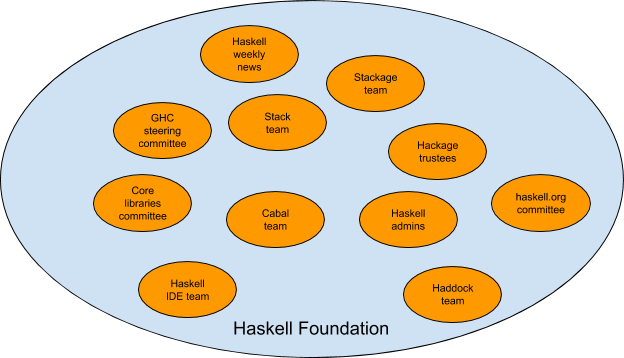
\includegraphics[scale=0.4]{community-glue.png}
	\end{center}

} 
\frame
{ 
	We fully launched with staff and all as of late February, 2021 (we're only 4 months old as of Tuesday!)
} 

\frame
{ 
	The board includes advisors from all over Haskell, consisting of well known community members, technical leaders, and even SPJ himself. See \href{https://haskell.foundation/who-we-are}{\blue{here}} for the full list. 
} 

\frame
{
	We discuss all of our goings on in three places: 
	
	\begin{enumerate}
		\item For formal board decisions, the \href{https://groups.google.com/u/2/a/haskell.foundation/g/board}{\blue{mailing list}}
		\item For formal working group discussions, the \href{https://discourse.haskell.org/c/haskell-foundation/11}{\blue{Haskell.org discourse}}
		\item For informal discussions, volunteer organizing, and general community, we have a \href{https://join.slack.com/t/haskell-foundation/shared_invite/zt-mjh76fw0-CEjg2NbyVE8rVQDvR~0F4A}{\blue{slack instance}}. 
	\end{enumerate}
}

\frame
{ 
	So far we have ~250 people engaging in volunteering, discussion, or otherwise helping out. 
} 

\subsection{Current status}
\frame
{ 
	\textbf{What's the current status of the Foundation?} 
} 

\frame
{ 
	Transparency time: We're doing well, but we can use help!
} 

\frame
{ 
	Volunteers help us do more things, faster. \textit{We are always actively seeking volunteers!}
} 

\frame
{ 
	Funding looks good so far, but more funding helps us do more things, for longer. 
} 

\frame
{ 
	If you'd like to get in contact with us about either, we have contact details \href{https://haskell.foundation/contact/}{\blue{on the website}}. 
	
} 

\subsection{What does the CTO do?}

\frame
{
	\textbf{What does "CTO" mean?} 

}

\frame
{ 
	My role is to help organize decisions regarding the Haskell ecosystem's technical landscape.
} 

\frame
{
	My duties include:
	
	\begin{itemize}
		\item Help to set the HF's technical agendas (the technical projects it works on).
		\item These can range from finding maintainers to support critical infrastructure, to 
		      funding projects (like GHC's CI setup), to blessing tech, to organizing new projects.
		\item Supporting existing tech is a priority, but in rare cases we'll try to "fill the gaps". 
		\item Educational materials are on the table too. 
    \end{itemize}	 

}


\frame
{
	Anyone can come to me anytime for info or direction. I'm happy to help. 
}

\section{Technical Agendas}
\frame
{ 
	Technical agendas for the HF vary widely, and touch many parts of the UX/DX for Haskell. 
}

\frame
{
  Agendas cover: 
  
  	\begin{itemize}
		\item Finding maintainers to support critical infrastructure
		\item Funding projects (like GHC's CI setup)
		\item Blessing new or existing tech
		\item Organizing new projects
		\item Educational materials  	
  	\end{itemize}

}

\frame 
{
		
	Supporting existing tech is a priority, but in rare cases we'll try to "fill the gaps". We acknowledge the hard work people are already doing! 

}

\frame
{
 	Decisions about what will be included are made by the HF's Technical Agenda working group. 
}

\frame
{ 
	We meet every Tuesday for a standup-style meeting. People are free to join. 
}

\frame
{
	Project announcements, RFC's, and community feedback are solicited on the Discourse. 
}

\frame
{ 
	Note: We may conflict with existing projects. This is a fact of life - we're not omniscient! When we solicit feedback on announcements or RFC's, if you tell us prior art exists, we'll evaluate it and see if we can support that instead. 
}

\frame
{ 
	This happened recently! See \href{https://discourse.haskell.org/t/proposal-unified-installer/2468/6?u=emilypi}{\blue{here}}
	
}

\section{Projects}
\subsection{Tech Projects}
\frame
{
	\textbf{We have 6 tech projects that we're working on now}
}

\frame
{ 
	\begin{enumerate}
		\item Utf-8 encoded Text by default 
		\item A Unified Haskell installer experience (thanks to the GHCup and Stack teams)
		\item Helping to fund GHC's CI setup
		\item Performance dashboards for GHC and core libraries
		\item Project Matchmaker 
		\item A book on performance tuning
	\end{enumerate}
}

\frame
{ 
	\begin{enumerate}
		\item Utf-8 encoded Text by default \textbf{(In Progress)}
		\item A Unified Haskell installer experience (thanks to the GHCup and Stack teams) \textbf{(In Progress)}
		\item Helping to fund GHC's CI setup \textbf{(Proposal Ready to Go)}
		\item Performance dashboards for GHC and core libraries \textbf{(In Progress)}
		\item Project Matchmaker \textbf{(In Progress)}
		\item A book on performance tuning \textbf{(Proposal almost ready)}
	\end{enumerate}
}

\subsection{How do we choose?}

\frame
{ 
	How do we choose ideas?
}

\frame
{ 
	How do we choose ideas? We ask you!
} 

\frame
{ 
	We also ask industry, and subject matter experts (like the GHC team)
} 

\frame
{ 
	When the working group votes to include something, we specify the project, and submit it to the Discourse for comment. If it looks good, we raise a proposal on the Tech Proposals repo in the \href{https://github.com/haskellfoundation}{HF github}. 
	
}

\subsection{Future Tech Projects}
\frame
{ 
	We have big plans in this area for the future. 
	
}

\frame
{ 
	Some ideas we plan on taking on: 
	
	\begin{itemize}
		\item An API for GHC
		\item Modernizing and improving HPC
		\item A community-led Haskell book (a la Rust book)
		\item Improved profiler tooling (I want Yourkit for Haskell!)
		\item Better error messages for GHC
	\end{itemize}
	
}

\subsection{Community Projects}
\frame
{ 
	We've been working on community efforts as well. 
}

\frame
{ 
	Theophile "Hecate" Choutri (aka Kleidukos, technoempress) has been immensely helpful with their time,
	contributing to documenting LITERALLY EVERYTHING.
}

\frame
{ 
	They're also working on \href{https://github.com/haskellfoundation/matchmaker}{Project Matchmaker}, a tool for developers to meet maintainers, and maintainers
	to put out a call for help. 
} 

\frame
{ 
	Hecate always needs help, so feel free to talk to them if you have free bandwidth. 
}

\frame 
{ 
	Book efforts: Gil Mizrahi is leading the Performance Tuning book efforts, and we'd love volunteers to help write content for it!
	
}

\frame
{ 
	We are partnering up with the Rust Foundation to help learn how to run good communities, and bring a common set of standards to all of our interactions with the community. 
}

\subsection{Future Community Projects}
\frame
{ 
	We have big plans for community events in the future as well. 
}

\frame
{ 
	Some ideas we plan on taking on: 
	
	\begin{itemize}
		\item An in-person conference for the Haskell community
		\item Ideas needed!
	\end{itemize}
} 

\subsection{Educational Projects}

\frame
{ 
	We have been in preliminary talks with some people from industry to help provide educational material (like Coursera etc.) to help bridge the gap between industry and hobbyist Haskell knowledge.
} 

\section{Funding Etc.}
\subsection{State of Funding}
\frame
{ 
	As stated above, we're doing okay with funding, but we would like to expand our efforts. 
} 

\frame
{ 
	We've done a lot for a company 4 months in the making. We'd like to do more. And we know we can!
} 

\frame
{ 
	We are aiming for a change in quality of life, but also a change in culture. 
} 

\frame
{ 
	What if we had the tools similar to other more modern languages? 

} 

\frame
{ 
	What if we had a glorious future for: 
	
	\begin{itemize}
		\item HLS. What if it had a stable API to work with? 
		\item Profiling tools. What if we had the ability to hook an agent into the RTS for live monitoring? 
		\item Coverage generation. What if it could extract to LCOV or other common formats?
		\item Debugging. What if we had a better way of debugging the heap? 
		\item Error messages. What if we had error messages that had levels of human readability?
	\end{itemize}
} 

\frame
{ 
	Think big! Not just what do we \textit{need}, but what do we \textit{want}?
} 

\subsection{Donating}

\frame
{ 
	Donations to the HF are finally in order. 
} 

\frame
{ 
	We accept individual donations now. See the donation button the HF website - you can set up recurring donations as well. 
} 

\frame
{ 
	For corporate donations, please get in touch with us at \blue{sponsorship@haskell.foundation}. 
} 

\frame
{ 
	Every little bit counts. 
} 

\frame
{ 
	As we funding rolls in, we'll have more leeway to work with marketing and branding to provide swag and merch. 
} 

\frame
{ 
	Individual donors will all get swag, it's just a matter of time and funding. 
} 

\frame
{ 
	Who doesn't want that sweet HF crop top and matching programming socks? 
} 

\subsection{Merch/Swag design}
\frame
{ 
	If you have designs you'd like to submit, we're happy to consider them.
} 

\frame
{ 
	Haskell's sticker game is LAME. I said it. 
} 

\frame
{ 
	If you've got an artist friend who'd like to help us, we would LOVE to talk to them. 
} 

\frame
{ 
	Supporting indie-artists is in the budget. 
} 

\section{Closing thoughts}

\frame
{ 
	Haskell is in a good place. I see a lot of optimism. 

}

\frame
{ 
	We're not out of the woods yet. There still are not as many people as I'd like to see working on critical infra. 
} 

\frame
{ 
	Ben Gamari deserves a special shoutout for being so incredibly helpful 
} 

\frame
{ 
	I'd also like to thank our volunteers and board members for donating their time. 
} 

\frame
{ 
	And of course, our corporate sponsors
} 

\frame
{ 
	\begin{center}
	
\includegraphics[scale=0.3]{sponsors.png}
	\end{center}
} 

\frame
{ 
	And, since we don't have their logos yet, Digital Asset and Exefreight.
} 

\end{document}